\documentclass[aspectratio=169]{beamer} %[aspectratio=169]
\usetheme{Boadilla}
\usecolortheme{seahorse}

\usepackage{parskip}

% հայկական և լատինական տառատեսակի կարգավորում
\usepackage{fontspec}
% \usepackage{polyglossia}
% \setdefaultlanguage{armenian}
% \newfontfamily\armenianfont{GHEA Mariam}
\setmainfont{DejaVu Serif}
\setsansfont{DejaVu Sans}
\setmonofont{DejaVu Sans Mono}
% \setmainfont{/home/srohund/Documents/1991/Arti Regular.otf}

% մաթեմի տառատեսակ
\usepackage{unicode-math}
% Set the math font to Fira Math

% Գույների համար
\usepackage{xcolor}
\definecolor{seahorseblue}{RGB}{0, 102, 204}
\definecolor{seahorsered}{RGB}{204, 0, 0}
\definecolor{seahorsegreen}{RGB}{0, 153, 0}
\definecolor{seahorseyellow}{RGB}{255, 204, 0}

\definecolor{seahorseblue2}{RGB}{0, 105, 148}
\definecolor{seahorsegreen2}{RGB}{0, 128, 71}
\definecolor{seahorsered2}{RGB}{217, 0, 27}
\definecolor{seahorseorange2}{RGB}{255, 123, 0}
\definecolor{seahorsegray2}{RGB}{92, 92, 92}
\definecolor{seahorsepink2}{RGB}{214, 0, 96}
\definecolor{seahorseyellow2}{RGB}{255, 201, 0}

% հղումների համար
\usepackage{hyperref}
\hypersetup{
	colorlinks=true,
	linkcolor=seahorsered,
	urlcolor=seahorseblue,
	citecolor=seahorsegreen,
}

% պատկերներ
\usepackage{graphicx}
\graphicspath{ {./images/} } % \includegraphics


% հատուկ հրաման մեջտեղում գրելու համար
\newcommand{\tabitem}{%
  \usebeamertemplate{itemize item}\hspace*{\labelsep}}

% հիմնական տվյալներ
\title[մաթ․ անալիզ - դաս 3]{1991 ստորաբաժանման դիմորդների նախապատրաստական դասընթաց}
\subtitle{Մաթեմաթիկական անալիզի ներածություն, դաս 3}
\author[Առաքելյան Ա․]{
    \href{mailto:aram.arakeljan@gmail.com}{Առաքելյան Արամ}
}
\institute{\href{https://1991.mil.am/}{«1991» ակադեմիա}}

\date{2023թ դեկտեմբեր}
\begin{document}
    % գլխարկ
    \begin{frame}
        \titlepage
	% \maketitle
    \end{frame}
%%%%% Նախորդ դասին %%%%%
    \begin{frame}
        \frametitle{Նախորդ դասերին}
        \centering
        Շուտով․․․
    \end{frame}
%%%%% Բովանդականություն %%%%%
    \begin{frame}
        \frametitle{Բովանդականություն}
        \centering
        Շուտով․․․
    \end{frame}
%%%%% 1 %%%%%
    \begin{frame}
        \frametitle{Զուգամետ հաջորդականություն}
        \framesubtitle{Սահման}
        \only<1-7>{
            \begin{block}{Սահմանում}
                Հաջորդականությունը կոչվում է \alert<1>{զուգամետ}, եթե ունի \alert<2>{սահման}։
            \end{block}
            \only<2>{\centering 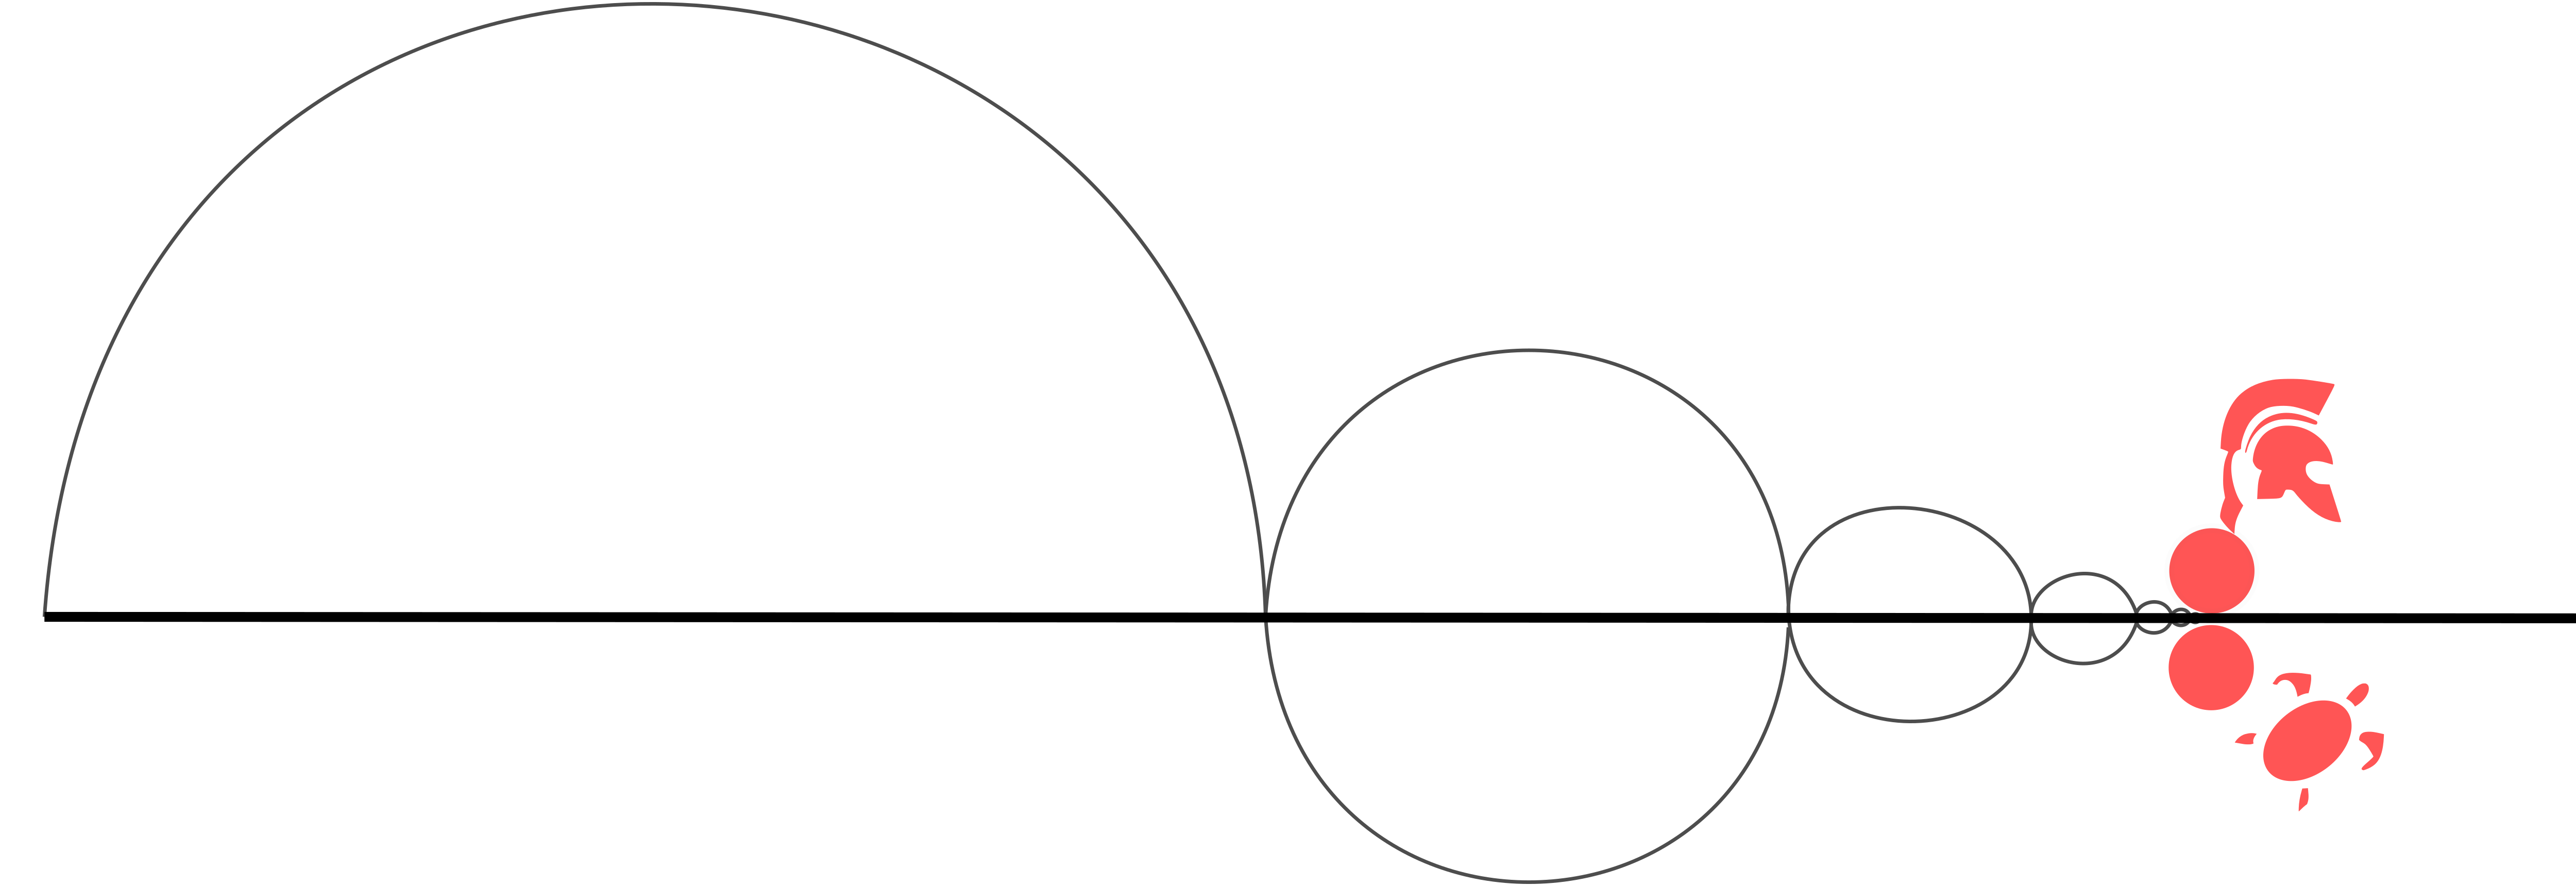
\includegraphics[width=0.5\textwidth]{zeno_achilles_paradox_i.png}}
        }
        \only<3-13>{
            \begin{block}{Սահմանում}
               \alert<9>{ $\alpha \in \mathbb{R}$} թիվը \alert<8>{$(a_n)$} հաջորդականության \alert<3>{սահմանն է}, եթե \only<-7>{\alert<5>{ինչքան ասես մոտիկ է $\alpha$ թվին}, \alert<6>{սկսած ինչ֊որ պահից}։}
                \only<4->{\[\alert<5, 10, 11, 13>{\forall \varepsilon > 0}\; \alert<6, 12>{\exists N_{\varepsilon} \in \mathbb{N}: \; \forall n > N_{\varepsilon}} \; \alert<5, 11>{|a_n - \alpha| < \varepsilon}:\]}
                \only<7>{Հաջորդականություն սահմանը նշանակվում է \alert<7>{$\lim_{n \rightarrow \infty}a_n$}-ով։}
            \end{block}
            \only<8>{\centering \includegraphics[width=0.42\textwidth]{5b49576b/convergent_sequence_0.png}}
            \only<9>{\centering \includegraphics[width=0.42\textwidth]{5b49576b/convergent_sequence_1.png}}
            \only<10>{\centering \includegraphics[width=0.42\textwidth]{5b49576b/convergent_sequence_2.png}}
            \only<11>{\centering \includegraphics[width=0.42\textwidth]{5b49576b/convergent_sequence_3.png}}
            \only<12>{\centering \includegraphics[width=0.42\textwidth]{5b49576b/convergent_sequence_4.png}}
            \only<13>{\centering \includegraphics[width=0.42\textwidth]{5b49576b/convergent_sequence_5.png}}
        }
        \only<14-41>{
            \begin{exampleblock}{Օրինակ}
               { $a_n = \sqrt[n]{n}$} հաջորդականության սահմանը $1$ է։
            \end{exampleblock}
        }
        \only<42-48>{
            \begin{exampleblock}{}
                $n!$ $n$ էլեմենտների տեղափոխության քանակն է։\\
                $4$ տարբեր խաղաքարտերը $4$ հոգուն կարելի է բաժանել $16$ եղանակով։
            \end{exampleblock}
        }
        \only<15-27>{
            \begin{alertblock}{Ապացույց}
                \only<15->{Պետք է ցույց տալ, որ սկսած ինչ֊որ պահից $|\sqrt[n]{n} - 1| < \varepsilon$։}
                \only<16>{\[|\sqrt[n]{n} - 1| < \varepsilon \Leftrightarrow - \varepsilon < \sqrt[n]{n} - 1 < \varepsilon\]}
                \only<17->{\[|\sqrt[n]{n} - 1| < \varepsilon \Leftrightarrow \alert<18, 23>{1-\varepsilon <} \alert<18, 23-24>{\sqrt[n]{n}} \alert<24>{< 1+\varepsilon}\]}
                \only<18->{Նկատենք, որ $\forall n \in \mathbb{N}\; \sqrt[n]{n} > 1$ \only<23->{ և հետևաբար \alert<23>{$1-\varepsilon < \sqrt[n]{n}$}:\\}}
                \only<19-22>{Դիցուք $\sqrt[n]{n} = x$, ապա $x^n = n$:\\}
                \only<20-21>{Եթե \alert<21>{$x<1$}, ապա $x^n = \alert<21>{x} \cdot x^{n-1} \alert<21>{< 1}\cdot x^{n-1}$:\\}
                \only<22>{Եթե $x<1$, ապա $x^n  < x^{n-1} < x^{n-2}< \cdots < x^{1} < 1$:\\}
                \only<25->{$\sqrt[n]{n} < 1 + \varepsilon$, այն և միայն այն դեպքում, երբ $\alert<26>{n} < (1+\varepsilon)^{\alert<26>{n}}$:\\}
                \only<27>{\[n < (1+\varepsilon)^n =?\]}
            \end{alertblock}
        }
        \only<28-39>{
            \begin{exampleblock}{Նյուտոնի երկանդամ}
                \only<28->{$(a+b)^2 = a^2 + 2ab + b^2$\\}
                \only<29-34>{$(a+b)^3 = \alert<31>{a^3} + 3\alert<32-35>{a^2b} + 3ab^2 + b^3$\\}
                \only<35->{$(a+b)^3 = a^3b^0 + 3\alert<32-35>{a^2b^1} + 3a^1b^2 + a^0b^3$\\}
                \only<30-34>{
                    $(a+b)^3 = 
                        (\alert<31, 32, 33>{a}+\alert<34>{b})
                        (\alert<31, 32, 34>{a}+\alert<33>{b})
                        (\alert<31, 33, 34>{a}+\alert<32>{b})$\\
                }
                \only<35>{
                    $(a+b)^3 = 
                    \textcolor{seahorseblue}{
                        \underbrace{(a+b)}_b
                    }
                    \textcolor{seahorsegreen}{
                        \underbrace{(a+b)}_a
                        \underbrace{(a+b)}_a
                    }$\\
                }
                \only<36-39>{$(a+b)^n = \underbrace{\textcolor<38>{seahorsegreen}{\textcolor<39>{seahorseblue}{(a+b)}\textcolor<39>{seahorsegreen}{(a+b)}}\cdots \textcolor<38-39>{seahorsegreen}{(a+b)}}_{n \text{ հատ}} = \alpha_{n, 0}\alert<37-38>{a^nb^0} + \alpha_{n-1, 1}\alert<39>{a^{n-1}b^1} + \cdots + \alpha_{0, n}a^0b^n$\\}
                \only<36-39>{Որտեղ $\alpha_{i, j}$֊ն $n$ հատ էլեմենտներից $i$ հատը ընտրելու տարբեր եղանակների քանակն է։}

            \end{exampleblock}
        }
        \only<40->{
            \only<-41, 49->{\begin{exampleblock}{$n$ հատից $i$ հատը ընտրել}
                \only<40->{$n$ հատ էլեմենտներից $i$ հատը ընտրելու եղանակների քանանակը հավասար է}
                \only<41>{\[\frac{n!}{i!(n-i)!},\] որտեղ $n! = 1 \cdot 2 \cdot 3 \cdots n$։}
                \only<49->{
                    \only<-49>{$n$ հատ էլեմենտների տեղափոխությունների քանակը հարաբերած $i$ և $n-i$ հատ էլեմենտների տեղափոխությունների քանակների արտադրյալին.}
                    \[C_n^i \equiv \binom{n}{i} := \frac{n!}{i! (n-i)!}\]
                }
            \end{exampleblock}}
            \only<42>{\centering \includegraphics[width=0.75\textwidth]{5b49576b/permutations_s1_e0.png}}
            \only<43>{\centering \includegraphics[width=0.75\textwidth]{5b49576b/permutations_s2_e0.png}}
            \only<44>{\centering \includegraphics[width=0.75\textwidth]{5b49576b/permutations_s2_e3.png}}
            \only<45>{\centering \includegraphics[width=0.75\textwidth]{5b49576b/permutations_s3_e0.png}}
            \only<46>{\centering \includegraphics[width=0.75\textwidth]{5b49576b/permutations_s3_e11.png}}
            \only<47>{\centering \includegraphics[width=0.75\textwidth]{5b49576b/permutations_s4_e0.png}}
            \only<48>{\centering \includegraphics[width=0.75\textwidth]{5b49576b/permutations_s4_e23.png}}
            %% p
            \only<50>{\centering 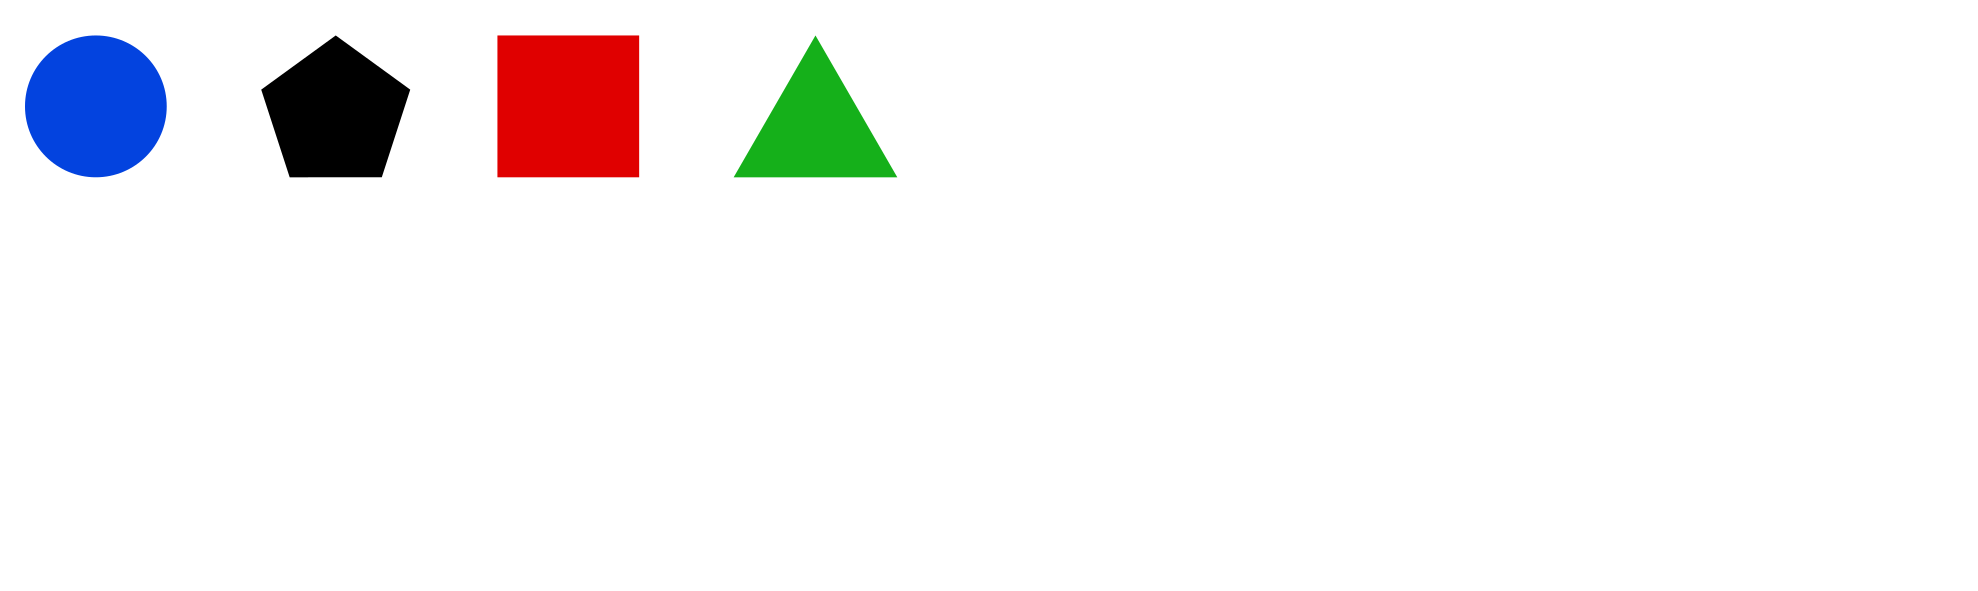
\includegraphics[width=0.35\textwidth]{particular_choice_0.png}}
            \only<51>{\centering 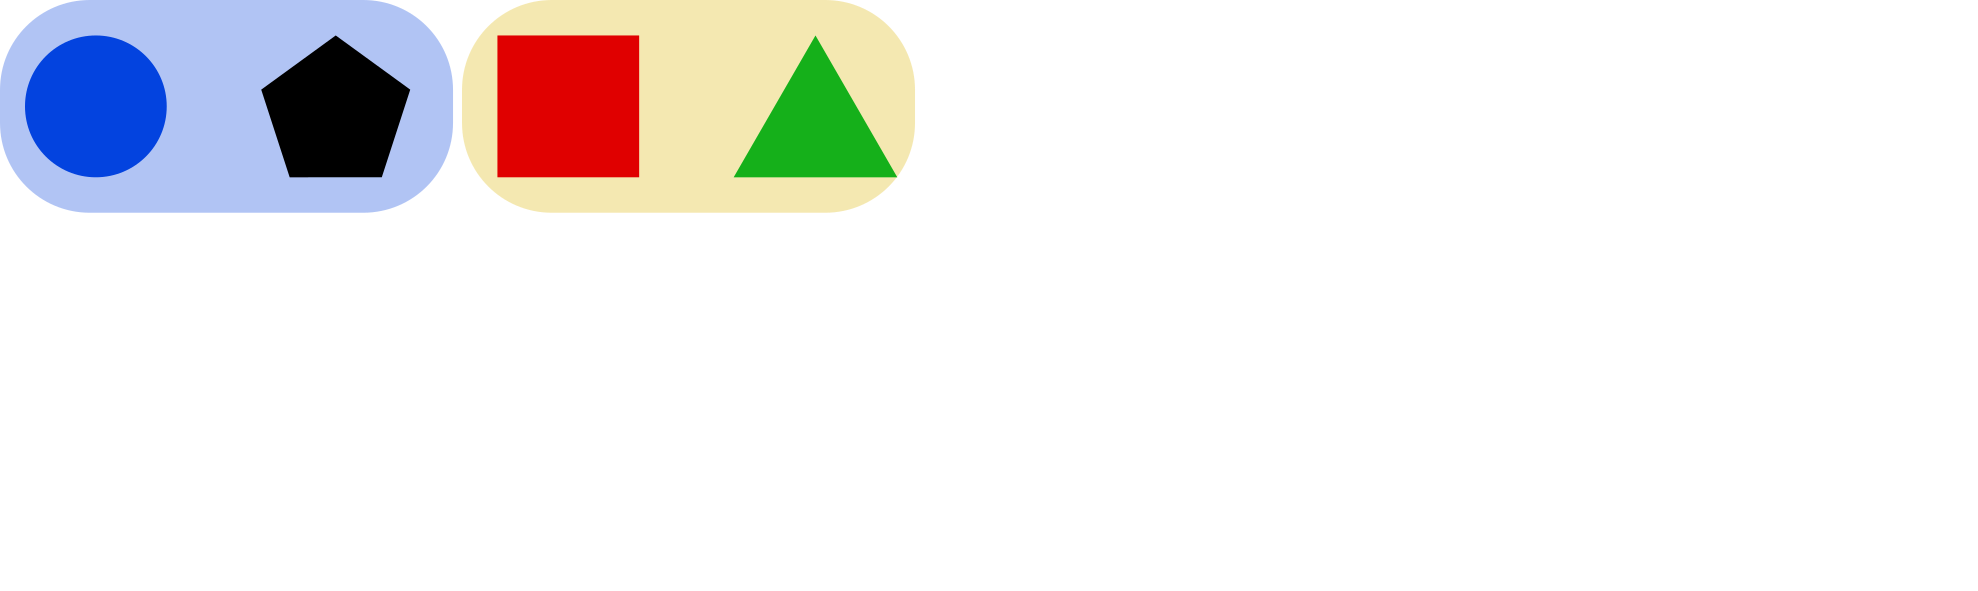
\includegraphics[width=0.35\textwidth]{particular_choice_1.png}}
            \only<52>{\centering 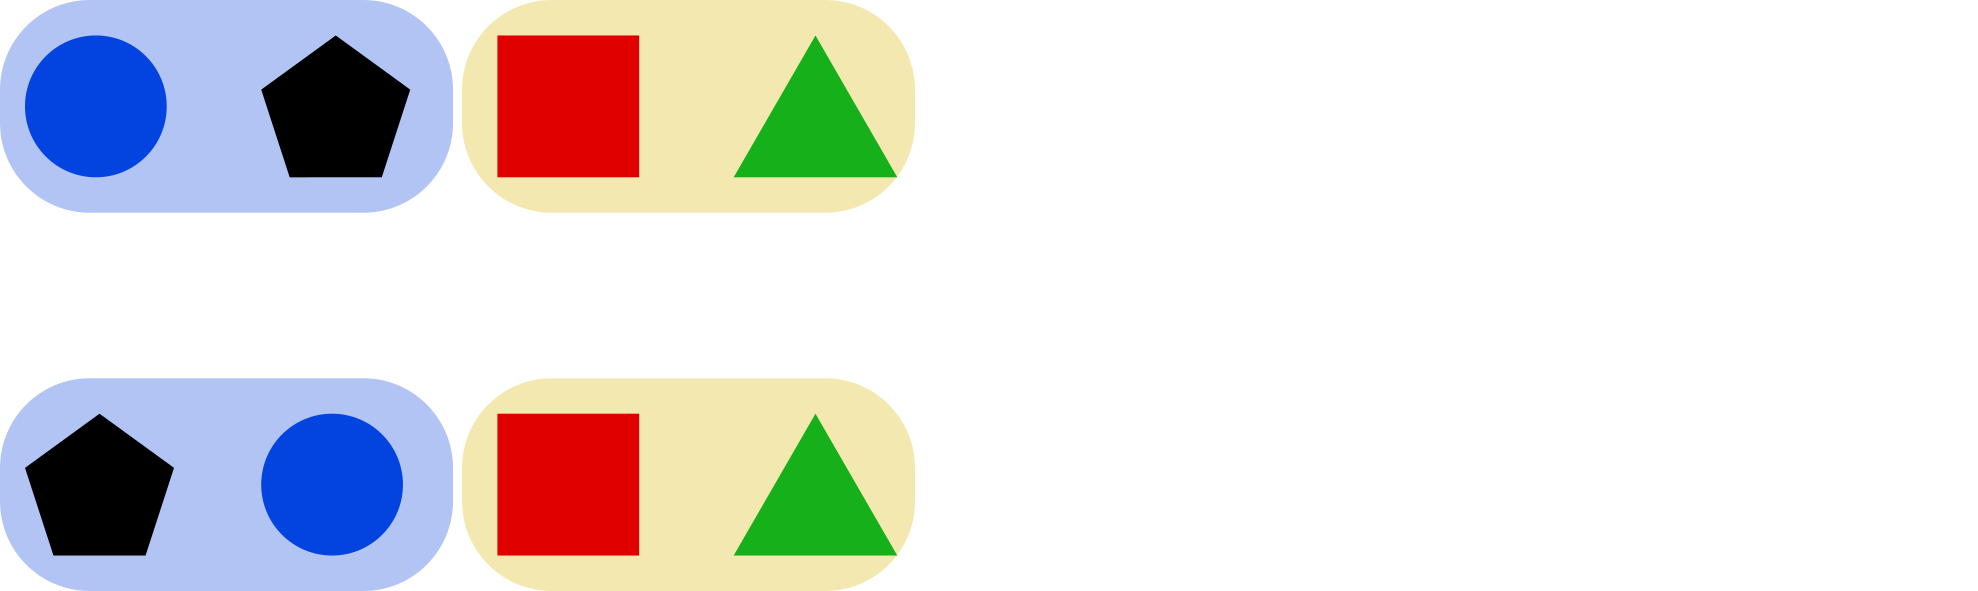
\includegraphics[width=0.35\textwidth]{particular_choice_2.png}}
            \only<53>{\centering 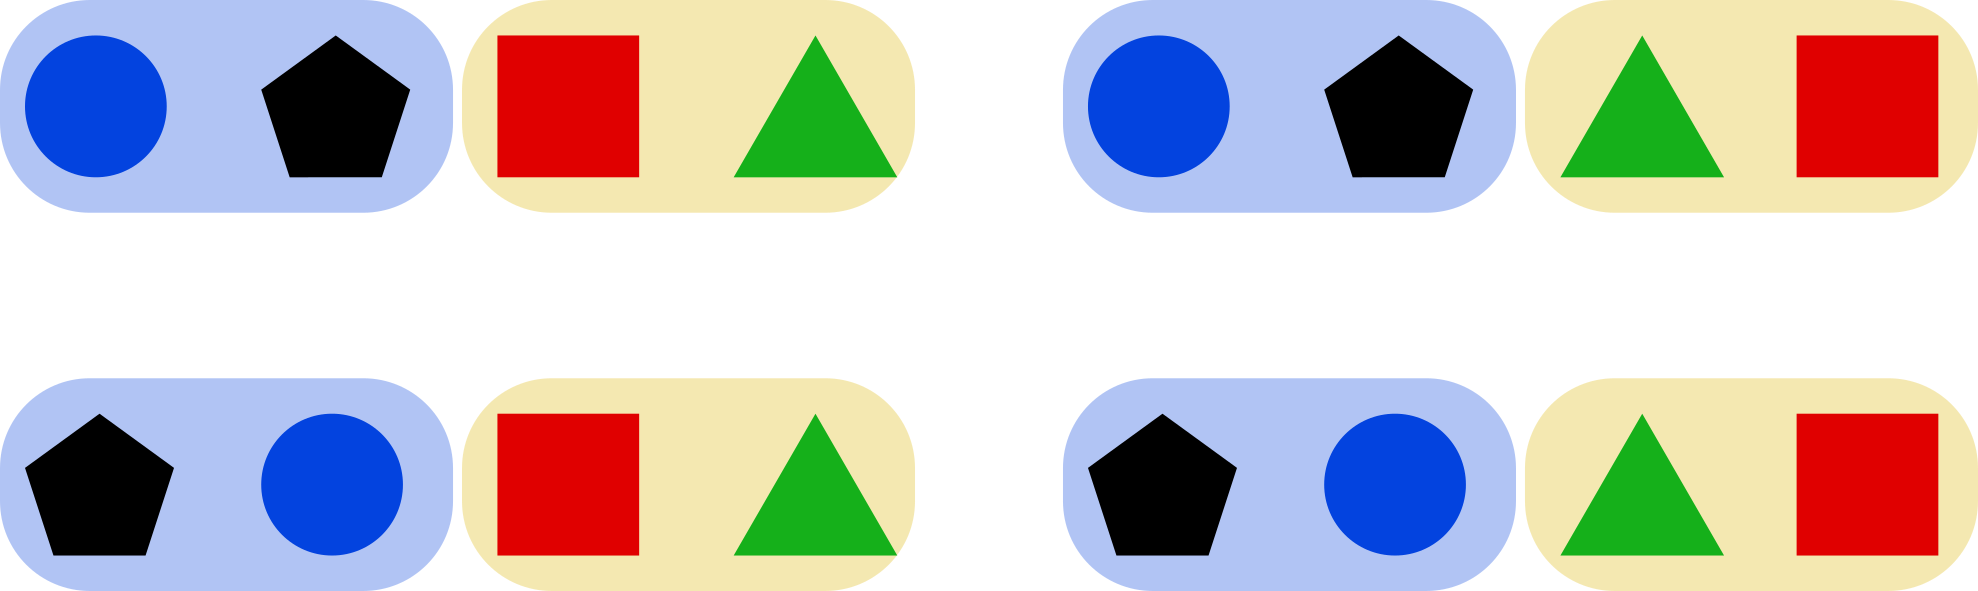
\includegraphics[width=0.35\textwidth]{particular_choice_3.png}}
            \only<54>{\centering 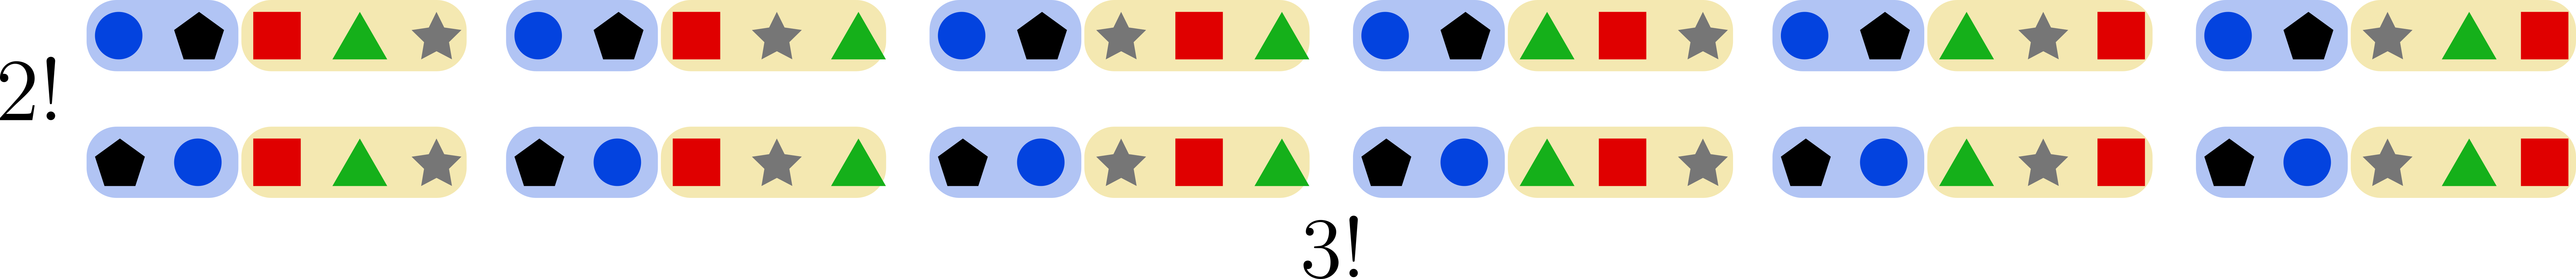
\includegraphics[width=0.85\textwidth]{particular_choice_m_0.png}}
        }
    \end{frame}
%%%%% 2 %%%%%
    \begin{frame}
        \frametitle{Զուգամետ հաջորդականություն}
        \framesubtitle{Ֆունդամենտալությունը}
        \only<1-3, 10->{
            \begin{block}{Պնդում}
                Զուգամետ Հաջորդականությունը ֆունդամենտալ է։
                \only<2-4>{Այսինքն՝ \[\forall \varepsilon > 0 \; \exists N_\varepsilon \in \mathbb{N}: \; \forall n, m > N_\varepsilon \; |a_n - a_m| < \varepsilon:\]}
            \end{block}
        }
        \only<3->{
            \begin{alertblock}{Ապացույց}
               \only<3->{Դիցուք $(a_n)$ հաջորդականությունը սահմանը $\alpha \in \mathbb{R}$ է, ինչ֊որ պահից սկասած }\only<4-9>{...}
               \only<10->{\alert<15>{$|a_n - \alpha| < \frac{\varepsilon}{2}$} և \alert<15>{$|a_m - \alpha| < \frac{\varepsilon}{2}$}։}
               \only<11>{\[|a_n - a_m|\]}
               \only<12>{\[|a_n - a_m| = |a_n - a_m + \alert{\alpha - \alpha}|\]}
               \only<13>{\[|a_n - a_m| = |(a_n - \alpha) + (\alpha - a_m)|\]}
               \only<14>{\[|a_n - a_m| = |(a_n - \alpha) + (\alpha - a_m)| \leq |a_n - \alpha| + |\alpha - a_m| \]}
               \only<15>{\[|a_n - a_m| = |(a_n - \alpha) + (\alpha - a_m)| \leq \alert{\underbrace{|a_n - \alpha|}_{\text{փոքր է } \frac{\varepsilon}{2}}} + \alert{\underbrace{|\alpha - a_m|}_{\text{փոքր է } \frac{\varepsilon}{2}}}\]}
               \only<16>{\[|a_n - a_m| \leq \varepsilon\]}
            \end{alertblock}
            \only<4>{\centering \includegraphics[width=0.42\textwidth]{5b49576b/convergent_cauchy_0.png}}
            \only<5>{\centering \includegraphics[width=0.42\textwidth]{5b49576b/convergent_cauchy_1.png}}
            \only<6>{\centering \includegraphics[width=0.42\textwidth]{5b49576b/convergent_cauchy_2.png}}
            \only<7>{\centering \includegraphics[width=0.42\textwidth]{5b49576b/convergent_cauchy_3.png}}
            \only<8>{\centering \includegraphics[width=0.42\textwidth]{5b49576b/convergent_cauchy_4.png}}
            \only<9>{\centering \includegraphics[width=0.42\textwidth]{5b49576b/convergent_cauchy_5.png}}
        }
    \end{frame}
\end{document}